%ex15.tex

\section{Exercice 15 - Coloration de Sommets}\label{ex15}

\begin{center}
\begin{algorithm}[H]
\caption{Approximation de $\chi$(G) via les degr\'es des sommets}\label{ex15_algo}
\algsetup{indent=2em,linenodelimiter= }
\begin{algorithmic}[1]
\REQUIRE $G$ : graphe de n sommets
\ENSURE $\chi(G)$ : nombre de couleurs n\'ecessaires pour colorer G
\STATE $C = \emptyset$
\STATE $k = 0$ 
\STATE $d_1 >= d_2 >= ... >= d_n$ les degr\'es des sommets
\REPEAT
	\STATE $k = k+1$
	\STATE colorier le sommet x ayant le plus haut degr\'e avec k
	\STATE marquer les voisins de x
	\STATE $C = C \cup \{x\}$
	\WHILE {$\exists$ un sommet y non marqu\'e et non color\'e}
		\STATE colorier y ayant le plus haut degr\'e avec k
		\STATE marquer les voisins de y
	\ENDWHILE
	\STATE effacer toutes les marques
\UNTIL {tous les sommets sont color\'es}
\RETURN $k$
\end{algorithmic}
\end{algorithm}
\end{center}

\subsection{Question 1}\label{ex15_q1}
Soit la num\'erotation suivante (en fonction des degr\'es) :
%ex15_fig1.tex
%numerotation en fonction des degres de l'exemple

\begin{figure}[h]
	\begin{center}
	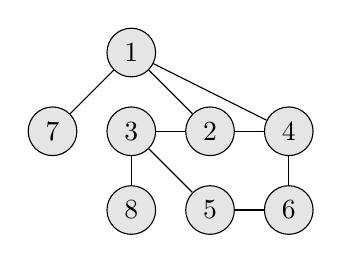
\begin{tikzpicture}
		\node[circle,draw=black,fill=black!10] (x1) at (0,0) {7};
		\node[circle,draw=black,fill=black!10] (x2) at (1,1) {1}
			edge[-] (x1);
		\node[circle,draw=black,fill=black!10] (x3) at (2,0) {2}
			edge[-] (x2);
		\node[circle,draw=black,fill=black!10] (x4) at (1,0) {3}
			edge[-] (x3);
		\node[circle,draw=black,fill=black!10] (x5) at (1,-1) {8}
			edge[-] (x4);
		\node[circle,draw=black,fill=black!10] (x6) at (2,-1) {5}
			edge[-] (x4);
		\node[circle,draw=black,fill=black!10] (x7) at (3,-1) {6}
			edge[-] (x6);
		\node[circle,draw=black,fill=black!10] (x8) at (3,0) {4}
			edge[-] (x3)
			edge[-] (x2)
			edge[-] (x7);
	\end{tikzpicture}
	\end{center}
	\caption{Numérotation en fonction des degrés}
	\label{ex15_fig1}
\end{figure}



En appliquant l'algorithme ci-dessus on obtient la coloration suivante :
%ex15_fig2.tex
%coloration de l'exemple avec l'algo
\begin{figure}[h]
	\begin{center}
	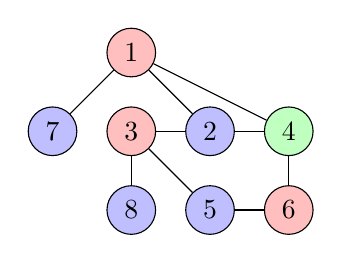
\begin{tikzpicture}
		\node[circle,draw=black,fill=blue!25] (x1) at (0,0) {7};
		\node[circle,draw=black,fill=red!25] (x2) at (1,1) {1}
			edge[-] (x1);
		\node[circle,draw=black,fill=blue!25] (x3) at (2,0) {2}
			edge[-] (x2);
		\node[circle,draw=black,fill=red!25] (x4) at (1,0) {3}
			edge[-] (x3);
		\node[circle,draw=black,fill=blue!25] (x5) at (1,-1) {8}
			edge[-] (x4);
		\node[circle,draw=black,fill=blue!25] (x6) at (2,-1) {5}
			edge[-] (x4);
		\node[circle,draw=black,fill=red!25] (x7) at (3,-1) {6}
			edge[-] (x6);
		\node[circle,draw=black,fill=green!25] (x8) at (3,0) {4}
			edge[-] (x3)
			edge[-] (x2)
			edge[-] (x7);
	\end{tikzpicture}
	\end{center}
	\caption{Numérotation en fonction des degrés}
	\label{ex15_fig2}
\end{figure}


% trace de l'algo

On remarque que sur cet exemple, la solution est \'egalement optimale : $\chi(G) = 3$.

\subsection{Question 2}\label{ex15_q2}
On doit trouver un graphe 2-colorable pour lequel l'algorithme renvoie n.\\
Prouvons qu'il n'en existe aucun.
Soit $G = (V,E)$ un tel graphe.\\
La seule mani\`ere pour que cet algorithme renvoie n, est qu'\`a chaque it\'eration, k
soit incr\'ement\'e, i.e. il ne doit jamais rentrer dans la boucle while.\\
Soit x le sommet de degr\'e maximum de G.\\
Si degr\'e(x)$ < n - 1$, alors soit y un sommet de G tel que $(x,y) \notin E$.
L'algorithme lui attribut alors la m\^eme couleur (1) que x (en passant dans le while).
Ne restant que n-2 sommets \`a colorer tout en ayant utilis\'e qu'une seule couleur,
l'algoritme renverra donc au plus n-1 couleurs. Ce qui est absurde par hypoth\`ese.\\
Donc degr\'e(x) = n-1.\\
Soit $G_2 = (V_2,E_2)$ le sous graphe de G priv\'e de x.\\
On note $x_2$ le sommet de degr\'e maximum de $G_2$.\\
Si $x_2$ n'est pas adjacent \`a tous les sommets non color\'es alors comme
pr\'ec\'edemment deux sommets poss\`ederont la m\^eme couleur. Ce qui emp\^echera
l'algorithme de renvy\'e n. $x_2$ est donc adjacent \`a tous les sommets de $G_2$, ie
degr\'e($x_2$) $>= n-2$.\\
Or x est adjacent \`a $x_2$ (cf plus haut), et donc degr\'e($x_2$) = n - 1.\\
En raisonnant de la m\^eme mani\`ere pour tous les sommets, nous arrivons donc \`a la
conclusion que G est le graphe complet \`a n sommets.\\
C'est \`a dire que G ne peut \^etre color\'e au mieux qu'avec n couleurs. Et donc lorsque
l'algorithme renvoie n, le graphe ne peut pas \^etre 2-colorable.

Par contre, il existe des graphes 2-colorables pour lequel l'algorithme renvoie
$\frac{n}{2}$, par exemple la couronne \`a n sommets (en supposant que la num\'erotation
des sommets fait les pires choix possibles) :
% !TEX root = ../main.tex
%ex15_fig3.tex
%couronne de taille 10

\begin{figure}[h]
	\begin{center}
		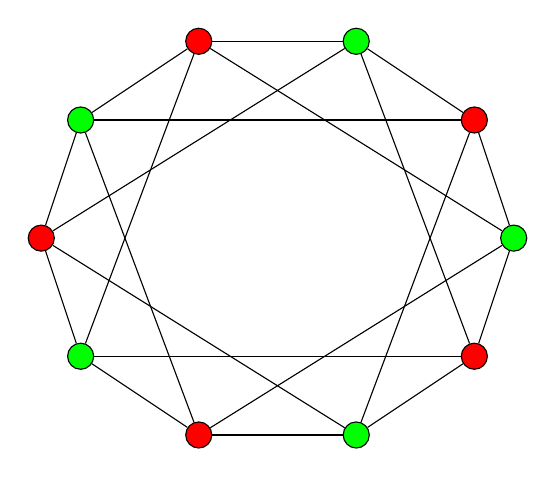
\begin{tikzpicture}
			\tikzset{node/.style={circle, draw=black}};
			\node[node,fill=red] (A) at (2,0) {};
			\node[node,fill=green] (B) at (4,0) {};
			\node[node,fill=green] (C) at (0.5,1) {};
			\node[node,fill=red] (D) at (5.5,1) {};
			\node[node,fill=red] (E) at (0,2.5) {};
			\node[node,fill=green] (F) at (6,2.5) {};
			\node[node,fill=green] (G) at (0.5,4) {};
			\node[node,fill=red] (H) at (5.5,4) {};
			\node[node,fill=red] (I) at (2,5) {};
			\node[node,fill=green] (J) at (4,5) {};

			\draw[black] (A) -- (B);
			\draw[black] (B) -- (D);
			\draw[black] (A) -- (C);
			\draw[black] (C) -- (E);
			\draw[black] (D) -- (F);
			\draw[black] (E) -- (G);
			\draw[black] (F) -- (H);
			\draw[black] (G) -- (I);
			\draw[black] (H) -- (J);
			\draw[black] (I) -- (J);
			
			\draw[black] (A) -- (G);
			\draw[black] (A) -- (F);
			\draw[black] (B) -- (H);
			\draw[black] (B) -- (E);
			\draw[black] (C) -- (D);
			\draw[black] (C) -- (I);
			\draw[black] (D) -- (J);
			\draw[black] (E) -- (J);
			\draw[black] (F) -- (I);
			\draw[black] (G) -- (H);
		\end{tikzpicture}
	\end{center}
	\caption{}
\end{figure}




